% % % % % % % % % % % % % % % % % % % % % % 
% dbi-intro.tex - Ian Huston
% $Id: dbi-intro.tex,v 1.66 2009/12/07 16:43:29 ith Exp $
% % % % % % % % % % % % % % % % % % % % % % 
% Redefine CVSRevision for this section
\renewcommand{\CVSrevision}{\version$Id: dbi-intro.tex,v 1.66 2009/12/07 16:43:29 ith Exp $}
% % % % % % % % % % % % % % % % % % % % % % % % % % % % % % % % 
% =========================================================== %
% % % % % % % % % % % % % % % % % % % % % % % % % % % % % % % % 
\chapter{Introduction to Dirac-Born-Infeld Inflation}
\label{ch:dbi-intro}
% % % % % % % % % % % % % % % % % % % % % % % % % % % % % % % % 
% =========================================================== %
% % % % % % % % % % % % % % % % % % % % % % % % % % % % % % % % 

% % % % % % % % % % % % % % % % % % % % % % % % % % % % % % % % 
% =========================================================== %
% % % % % % % % % % % % % % % % % % % % % % % % % % % % % % % % 
\section{Introduction}
% 
\label{sec:dbi-intro}
% % % % % % % % % % % % % % % % % % % % % % % % % % % % % % % % 
% =========================================================== %
% % % % % % % % % % % % % % % % % % % % % % % % % % % % % % % % 


The inflationary scenario provides the 
theoretical framework for the early history 
of the universe. It has now been successfully tested by observations, 
including the five year data from WMAP
\cite{Komatsu:2008hk}. Despite this success, however, the high energy 
physics that resulted in a phase of accelerated expansion is still 
not well understood. String and M-theory attempt to unify the fundamental
interactions 
including gravity. 
The early universe provides a unique window into high energy physics at scales currently
unreachable by particle accelerators.
It is therefore important to 
develop inflationary models within string theory and to confront them with 
cosmological observations.

 

One class of string theory models that has received 
considerable attention is D-brane inflation
\cite{brane1,brane2,brane3,brane4,brane5,
brane6,brane7,brane8,brane9,brane10,brane11,brane12,brane13,
brane14,brane15,brane16,brane17,Brodie:2003qv,Vikman:2006hk, 
Mukhanov:2005bu,Kallosh:2007wm,brane18,
brane19,brane20,brane21}. 
(For some recent reviews, see
\cite{tyereview,cline,McAllister:2007bg,Lorenz:2007ze,
Bean:2007eh,bean}). 
% Of particular interest 
% is the Dirac-Born-Infeld (DBI) inflationary scenario \cite{brane6,brane11}.
The Dirac-Born-Infeld (DBI) scenario 
of the compactified type IIB theory is a well-motivated model \cite{brane6,brane11}, 
in which inflation is driven by one or more ${\rm D}$-branes 
propagating in a warped ``throat'' background. 
% 
In the simplest version of the scenario, 
the inflaton parametrises the radial 
position in the throat of a single ${\rm D3}$-brane. 
The brane dynamics are determined by the DBI action in such a 
way that the inflaton's kinetic energy is bounded from above by the warped 
brane tension. The regime where this bound is nearly saturated is 
known as the ``relativistic'' limit.

% % % % % % % % % % % % % % % % % % % % % % % % % % % % % % % 
% ========================================================= %
% % % % % % % % % % % % % % % % % % % % % % % % % % % % % % %
% Intro from multibrane paper, removed but could be useful.
% % % % % % % % % % % % % % % % % % % % % % % % % % % % % % % % 
% The quest to realise inflation within string/M-theory continues to 
% attract considerable attention. The Dirac-Born-Infeld (DBI) scenario 
% of the compactified type IIB theory is a well-motivated model, 
% in which inflation is driven by one or more ${\rm D}$-branes 
% propagating in a warped `throat' background
% \cite{brane1,brane11,brane12,brane13, brane2,brane20,brane3, brane4,brane5,brane6}
% . Such a background is generated 
% by the non-trivial form-field fluxes over the internal dimensions. 
% (For recent reviews, see
% \cite{tyereview,McAllister:2007bg,Lorenz:2007ze,Kallosh:2007wm,Bean:2007eh,bean,
% cline}.) 
% In the simplest version of the scenario, 
% the inflaton parametrizes the radial 
% position in the throat of a single ${\rm D3}$-brane. 
% % % % % % % % % % % % % % % % % % % % % % % % % % % % % % % % 





In Part~\ref{part:dbi} of this thesis we will 
explore the observational consequences of DBI inflation. 
In general, primordial gravitational wave fluctuations
and non-Gaussian statistics in the curvature perturbation provide 
two powerful discriminants of inflationary scenarios. 
The nature of the DBI action is such that the sound 
speed of fluctuations in the inflaton can be much less than the speed of 
light. This induces a large and potentially detectable non-Gaussian 
signal in the density perturbations \cite{brane6,brane11,lidser3,chenetal}. 


In this chapter we introduce string theory, warped compactifications and DBI inflation.
In Chapter \ref{ch:dbi} we will derive upper and lower 
limits on the amplitude of the tensor perturbations.  
We will explore how these bounds may be relaxed in Chapter \ref{ch:multibrane} and discuss
multi-brane 
scenarios which permit observable tensor signals. 

% % % % % % % % % % % % % % % % % % % % % % % % % % % % % % % % 
% =========================================================== %
% % % % % % % % % % % % % % % % % % % % % % % % % % % % % % % % 
\section{String Theory and Extra Dimensions}
\label{sec:extradims}
% % % % % % % % % % % % % % % % % % % % % % % % % % % % % % % % 
% =========================================================== %
% % % % % % % % % % % % % % % % % % % % % % % % % % % % % % % % 
The desire to unify seemingly disparate theories has been a driving force in
theoretical physics for more than a hundred years. This effort has produced 
the Standard Model (SM) of particle physics which unifies three of the four
fundamental forces in a robust theoretical framework. Since the realisation of
the SM, a clear goal of theoretical physics has been the unification of the
fourth force---gravity---into this framework. String theory is one of the leading
contenders for achieving this unification. 
In this section we will introduce
some of the string theory concepts that will be required later to understand DBI
inflation.
Many review articles and text books have been written about string theory and
its application to cosmology and a short list of recent works includes
Refs.~\cite{cline, Johnson2000, Baumann:2009ni,Kallosh:2007wm,
Linde:2005dd,McAllister:2007bg}.


In string theory there are two main
types of strings, referred to as closed and open. These are distinguished by the fact
that closed
strings form a continuous loop while open strings have two unconnected ends. 
% The physics of their interactions dictates the physics of the SM which has
% been
% so successfully tested.
% 
% This at least is the goal of the string theory project but the complex nature
% of the mathematical and physical structures involved means that no single
% well-defined theory can claim to have achieved this goal. Indeed many
% different
% string theories have been discovered. This might appear to be a significant
% set-back in the attempt to find a single unifying theory. 
There are several different string theories which are linked in pairs by a process
called
duality. Physical descriptions in one theory can be translated into a
dual description in the other. The dual version often exhibits properties that
are useful for solving problems in the original setting.
% These dualities have demonstrated the existence of an underlying theory of
% which the individual string theories are only facets. 
We will work in the framework of the Type IIB theory since this has proven
to be the most
fruitful for generating models of cosmological inflation \cite{cline,
Linde:2005dd}. 
% 
% The most striking prediction of string theory is the existence of other
% dimensions beyond the four spacetime dimensions that we
% experience. Recovering the physics of our familiar $3+1$ dimensional universe
% clearly requires that these extra dimensions be hidden in some way. How this
% is
% achieved is one of the signature features of any complete string theoretical
% description of the universe.

% \subsection{Cosmology and String Theory}
% \label{sec:stringcos-dbiintro}
% % 
% Temperatures in the early universe were far in excess of those attainable by
% any earth-bound particle accelerator today. Hence, a stringent test of any high
% energy
% theory is whether it predicts the same properties of the early universe that are
% now being observed in the CMB and elsewhere.
% % For this reason any string theory description of the universe must include a
% % consistent cosmological narrative. 
% % 
% In Chapter \ref{ch:introduction} inflation was put forward as the leading
% scenario for the evolution of the early universe. For string theory to
% be
% a consistent framework for the inflationary paradigm, it must produce a period of
% inflationary expansion. Although inflation is usually described by SM scalar
% fields, there is no
% evidence yet for the existence of such fields in the SM. Higher
% energy theories such as string theory could provide an explanation for the
% existence of inflaton fields.
% %  In this way inflation and string theory are
% % ideal partners and it is natural to consider them together when investigating
% % the early universe.
% 
% 
% Cosmology can be used as a tool to constrain string theory. Much of the evidence
% of an
% era of string theory physics would be removed by a period of inflation, but the
% observational results of inflation itself could provide clues about the nature
% of such an era. 
% 
% One avenue of investigation would be to look for signals that are generic in string theory and
% see if they are observed. While this could not definitively prove string theory to be the 
% cause it would vindicate continued efforts to prove the theory is consistent
% with observations. Conversely any observed
% signal that is predicted to occur rarely in string theory would make the theory more implausible.
% % Limiting the parameter space of an acceptable string theory to an ever smaller
% % region would also
% % decrease its viability even if it could not be ruled out. 
% One observational parameter suited to this is the non-Gaussianity
% parameter $\fnl$ as introduced in Section~\ref{sec:fnl-intro}.
% Standard inflation models, including the single field slow roll model described in
% Section~\ref{sec:slowroll-intro}, produce small amounts of $\fnlloc$, whereas
% certain classes of string theory inspired models have large non-Gaussian
% signatures. 
% % While not exclusively a string theory effect, a detection of or
% % failure to detect non-Gaussianity would rule in and out large classes of
% % models.

\subsection{Extra Dimensions}
String theory predicts that the one time-like and three spatial dimensions that
constitute the observable universe do not represent the complete spacetime manifold.
Instead,
our universe is a 10 or
11 dimensional spacetime and physical theories in 3+1 dimensions must
therefore be able to explain why the 
other 6 or 7 dimensions are unobservable. One of the challenges of string
theory is how 
to ``hide'' these extra dimensions in such a way as to 
recover the standard four-dimensional cosmology at low energies.

The early work of Kaluza and Klein (KK) in formulating higher dimensional 
theories laid the groundwork for the current treatment of extra dimensions in
string theory \cite{Kaluza1921, Klein1926}. By
compactifying an extra dimension onto a circle of finite radius an infinite
tower of extra fields are introduced into the lower dimensional theory. The
mass of these fields is inversely proportional to the size of the extra
dimension. The appearance of these
unobserved massive fields is avoided by taking the radius to be extremely small.
This leaves a
massless degree of freedom which must be accounted for in the four-dimensional
effective action. 


A similar procedure is undertaken when compactifying string theory from a
10 or 11 dimensional description down to four dimensions (for reviews see
Refs.~\cite{douglas,grana}).
In ten dimensional type IIB theory the six extra dimensions are
compactified into a Ricci flat Calabi-Yau (CY) manifold which can be described
by three complex coordinates \cite{Yau1977}. 
Because any Ricci flat metric can be
rescaled onto another Ricci flat metric, there is no unique solution for the
metric on the CY manifold. Instead a family of solutions exists with many free
parameters. These parameters remain after the compactification, in
analogy to the size of the extra dimension in KK compactification, and can depend
on position in the four-dimensional spacetime. They appear as fields
in the four-dimensional theory and are known as moduli. 
These fields are not subject to any symmetry and so their individual values
at different spacetime points can affect the physics at those points.





% Suppose we wish to reduce a theory in $(D+1)$ dimensions to one in
% $D$ dimensions. 
% We will ``compactify'' the 
% (here single) extra dimension on a circle of finite radius $L$ and
% denote the coordinate on the circle as $z$. 
% Assume that in $(D+1)$ 
% dimensions we have a metric tensor $\hat{g}_{MN}(x,z)$ where $M$ and
% $N$ run over all $(D+1)$ dimensions and 
% x signifies the $D$ coordinates of the lower-dimensional spacetime.
% Hats  denote quantities in the $(D+1)$ spacetime.
% A Fourier decomposition of $\hat{g}_{MN}$ gives an infinite number
% of fields in $D$ dimensions:
% \begin{equation}
%  \hat{g}_{MN}(x,z) = \sum_n g_{MN}^{(n)}(x) e^{i\frac{nz}{L}}\,.
% \end{equation}
% The mode number $n$ is related to the mass of the resulting fields;
% modes with $n=0$ will be massless and those with
% $n \ne 0$ massive. This can be seen by considering the Klein-Gordon
% equation for a $(D+1)$ dimensional field $\hat{\varphi}$:


\subsection{T-duality}
\label{sec:tduality-dbiintro}
% T-Duality
In string theory an extra space time symmetry is present which relates physical properties in
theories with large compactification radius with those in theories with small radius. 
Suppose we have a string theory compactified on a circle of radius $L$. The ``T-duality''
transformation which relates two physical theories with this one compactified dimension is
% 
\begin{equation}
\label{eq:tdualtransform-dbiintro}
 L \rightarrow \wt{L} = \frac{\alpha'}{L}\,.
\end{equation}
% 
Now consider what effect this transformation will have on the momentum of a closed string. Instead
of being a continuum, the momentum takes discrete values
$j/L$ for $j \in \mathbb{Z}$. This is a KK tower of massive states. As we
complete a circuit around the compact dimension, the value of the coordinate
function embedding the string in the background will increase by $2\pi w
L$ for $w \in \mathbb{Z}$. This $w$, called the winding number of the string,
can only be non-zero for closed strings, which can be wrapped around the periodic
dimension.

The total mass of the string contains terms with both the KK tower of states
and the new tower of winding states:
\begin{equation}
\label{eq:closedmass-dbiintro}
 M^2 = \frac{j^2}{L^2} + \frac{w^2 L^2}{\alpha'^2} + \cdots\,,
\end{equation}
where the string parameter $\alpha'$ is related to the string mass scale by
$\alpha'=1/\ms^2$.
If $L$ is taken to infinity, the $w\ne 0$ states become infinitely massive and
only the $w=0$ state is left with a continuum of momentum values. Thus, the
uncompactified result is recovered. However, if $L\rightarrow0$, the $j\ne 0$
states are now infinitely massive as in the standard KK picture. Unlike the
standard case, there is now a continuum of winding states with $w\ne 0$,
again giving an
uncompactified dimension. This major departure from the standard
compactification result is a purely stringy effect. 

The formula for the mass spectrum, \eq{eq:closedmass-dbiintro}, is invariant
when $j$ and $w$ are exchanged given the transformation in \eq{eq:tdualtransform-dbiintro}.
Writing the equations of motion in terms of $\wt{L}$, having interchanged $j$ and
$w$, gives a new theory which is compactified on a circle of radius $\wt{L}$. This is known as the
T-dual theory \cite{Sakai1986,Kikkawa1984b}. The two
theories are physically identical since T-duality is an exact symmetry
of string theory for closed strings. The T-duality applies to all physics in the theory and in
particular also affects open string modes. These behave in a different way under T-duality to closed
strings as will be described below.

% 
\subsection{D-Branes}
\label{sec:dbranes-dbiintro}
% Despite using string theory we will not be dealing with strings themselves.
The dynamics of extended objects known as branes are particularly important for
building inflationary models.
As mentioned in Section~\ref{sec:tduality-dbiintro}, string
theories are linked by T-duality. Fundamental parameters such as the size of the
extra-dimensions, the string coupling and the
coordinate solutions of the strings are related by such a symmetry.


We introduced T-duality by explaining
its effects on closed strings. But what happens to the open strings in a T-dualised theory? Open
strings, as their name suggests, have two open ends and
consequently cannot have a conserved winding number such as $w$. Suppose once more
that one
of the $D$ dimensions is compactified. As $L\rightarrow0$, the non-zero momentum
states become infinitely massive, but in contrast to the closed case there is now
no continuum of winding states. Thus, the open string now lives in $D-1$ dimensions
similar to the result of standard KK compactification \cite{Johnson2000}.
The endpoints of the open strings 
then observe Dirichlet boundary conditions, taking fixed values in the compactified
direction.
There are still closed strings in this theory, however, and these continue to
move in the full $D$ dimensions after being T-dualised.  

The result is similar if more than
one coordinate is made periodic.
If $D-p-1$ spatial dimensions are compactified, for some $p$, then the ends of
the open
strings can still move freely in the other $p$ spatial dimensions on a $p+1$
dimensional hypersurface. This hypersurface is called a Dirichlet brane or
D$p$-brane. The closed string modes move in the full $D$ dimensions.
% 
In Type IIB theory with supersymmetric strings, an extra condition implies that
only D$p$-branes with $p=1,3,5,7,9$ are stable\footnotemark.
\footnotetext{There is also a $p=-1$ D-instanton in which the time direction
along with all spatial directions is subject to Dirichlet boundary conditions
\cite{Green1992,Green1988,Green1977}.}
% 

D$p$-branes can be considered as dynamical objects in their own right with a
tension given by \cite{Johnson2000}\footnote{$T_p$ here is $\tau_p$ in
\Rref{Johnson2000}.}
% 
\begin{equation}
\label{eq:branetensiondefn-dbiintro}
 T_p = \frac{\ms^{p+1}}{(2\pi)^p \gs}\,,
\end{equation}
% 
where $\gs$ is the string coupling and $\ms$ is the string mass scale.
Their dynamics is governed by the action 
% 
\begin{equation}
\label{eq:gendbiaction-dbiintro}
 S_\mathrm{DBI} = -T_p \int \d^{p+1}\xi \sqrt{-\hat{g}}\,,
\end{equation}
where $\hat{g}_{ab}$ is the induced metric on the brane with internal
coordinates $\xi^a$, for $a=0,\ldots,p$, given by \cite{Johnson2000}
% 
\begin{equation}
 g_{\mu\nu} = \hat{g}_{a b} \frac{\partial \xi^a}{\partial x^\mu} \frac{\partial \xi ^b}{\partial x^\nu}\,.
\end{equation}
% 
\eq{eq:gendbiaction-dbiintro} is the general form of the DBI
action which will be used later.


In the simplest versions of slow roll inflation, only a single scalar field
with a
sufficiently flat potential is required to satisfy the slow roll conditions outlined
in
Section \ref{sec:slowroll-intro}. Since D-branes are charged (with Ramond-Ramond
charge), a D-brane and an anti-D-brane
($\overline{\mathrm{D}}$) separated by some distance will be attracted to each other.
The separation distance
can be identified as a scalar degree of freedom and under appropriate conditions
could play the role of the inflaton
field \cite{brane1,brane2,brane3,brane7,Brodie:2003qv,brane9}. 

As described above, compactifying dimensions
introduces scalar fields known as moduli. These fields must be
accounted for in the dynamics unless some way can be found to stabilise them by
fixing their masses to be large.
Initial efforts to induce inflation using D-branes ignored the issue of moduli
stabilisation. Instead, it was
assumed that whatever stabilisation mechanism was used would have no discernible
effect on the inflationary physics. Kachru \etal \cite{brane4} recognised that
in fact stabilisation will be important and must be taken into account.

% % % % % % % % % % % % % % % % % % % % % % % % % % % % % % % % % % % % % % % %
\subsection{Warped Throats}
\label{sec:warpedthroats-dbiintro}
% % % % % % % % % % % % % % % % % % % % % % % % % % % % % % % % % % % % % % % % 
The moduli must
be stabilised so that they do not appear in the effective action as
massless fields. This can be achieved by switching on background fluxes in the
compactified space. These fluxes are analogous to magnetic
fields in the higher dimensional space. By Gauss' theorem  the compact space
will now have a quantised non-zero total charge.
In the presence of fluxes, a general form for the ten dimensional metric is
\cite{Baumann:2009ni}:
\begin{equation}
\label{eq:warpedmetric-dbiintro}
 \d s^2 = e^{2A(y)}\eta_{\mu\nu} \d x^\mu \d x^\nu + e^{-2A(y)} g_{mn}\d y^m
\d y^n\,,
\end{equation}
where the function $A(y)$ varies across the compact dimensions $y^m$.
Compactifications in which $A$ varies significantly with $y$ are called warped
compactifications and $e^{A(y)}$ is referred to as the warp factor. These warped
compactifications are qualitatively similar to
the Randall-Sundrum scenario \cite{Randall1999,Brummer2006}.


Flux compactification of type IIB string theory to four dimensions 
results in such a warped geometry, where the six-dimensional CY  
manifold contains one or more throats \cite{douglas,gkp,grana}. 
The metric inside a throat takes the same form as in
\eq{eq:warpedmetric-dbiintro}:
% 
\begin{equation}
\label{eq:conemetric-dbiintro}
\d s_{10}^2= h^2 ( \rho) \d s_4^2 + h^{-2} (\rho ) 
\left( \d\rho^2 +\rho^2 \d s_{X_5}^2 \right) \,,
\end{equation}
%  
where the warp factor $h (\rho)$ is a function of the 
radial coordinate $\rho$ along the throat and $X_5$
is a Sasaki-Einstein five-manifold. 


In many cases, the ten-dimensional metric (\ref{eq:conemetric-dbiintro}) can be 
approximated locally by the geometry $AdS_5 \times X_5$, where the 
warp factor is given by $h=\rho /L$ and 
the radius of curvature of the $AdS_5$ space is defined by
%  
\begin{equation}
L^4 \equiv \frac{4\pi^4 \gs N}{{\rm Vol} (X_5) \ms^4} \,,
\end{equation}
% 
such that $\mathrm{Vol}(X_5)$ is the dimensionless volume of 
$X_5$ with unit radius and $N$ is the ${\rm D3}$  charge of the throat.


% In the bulk of the Calabi-Yau space $e^A \simeq 1$ so there is no warping. The
% SM brane could live here and not feel any effects of the warping.

In the Klebanov-Strassler (KS) background \cite{ks}, the throat 
is a warped deformed conifold and 
corresponds to a cone over the manifold 
$X_5 = T^{1,1}= {\rm SU(2)} \otimes {\rm SU(2)}/{\rm U(1)}$
in the UV limit ($\rho \rightarrow \infty$). This has   
a volume $\mathrm{Vol} (T^{1,1}) = 16\pi^3/27$ and  topology
$S^2\times S^3$, where the $S^2$ is fibred over the $S^3$.

\begin{figure}[htbp]
\centering
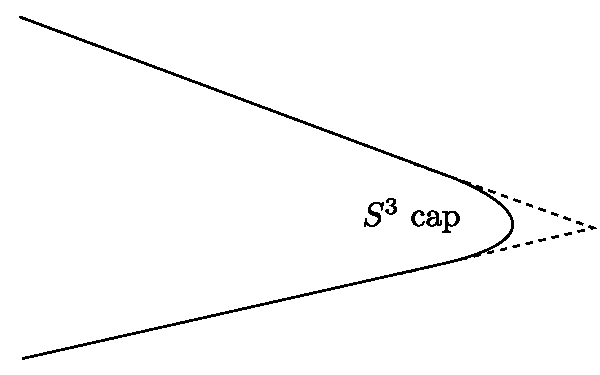
\includegraphics{dbi/graphs/deformed-conifold}   
\caption[Deformed Conifold]{A conifold can be deformed to remove the singularity at
the tip.}
\label{fig:conifold-dbiintro}
\end{figure}

There are two 3-cycles in the warped throat. The first is the $S^3$ subspace and
is known as the A-cycle. The second, called the B-cycle, is the $S^2$ times a
circle extended in the direction of the throat radius. The three-form fluxes
$F_3$ and $H_3$, aligned with these cycles, are turned on to make the warped
throat a solution of the Einstein equations \cite{cline}. The cycles are threaded with
quantised units of flux $M$ and $K$ given by: 
\begin{align}
\label{eq:fluxdefn-dbiintro}
 \frac{1}{2\pi\alpha'}\int_A F_3 &= M \,, \\
 \frac{1}{2\pi\alpha'}\int_B H_3 &= -K\,, 
\end{align}
where $M,K\in \mathbb{Z}$.
The D$3$ charge of the throat, $N$, is related to the quantised fluxes by
$N=MK$.
The wrapping of the fluxes along the cycles of the conifold smooths out the
conical singularity at the tip of the throat with an $S^3$ cap 
\cite{ks,kt}, as shown in Figure~\ref{fig:conifold-dbiintro}, and the warp factor
asymptotes to 
a constant value in this region.


In this section we have summarised the concepts that will be
required to discuss DBI inflation. The compactified warped throat described
here will provide the setting for this string theoretic realisation of
inflation. 
% In Section \ref{sec:stringcos-dbiintro} we outlined how cosmological
% observations can constrain the parameter space of string theories. 
In the next
section we connect the geometry and physics of the string compactification with
inflationary cosmology and establish the observational parameters that will directly
enable concrete constraints to be formulated. 

% 
% 
% % % % % % % % % % % % % % % % % % % % % % % % % % % % % % % % 
% =========================================================== %
% % % % % % % % % % % % % % % % % % % % % % % % % % % % % % % % 
\section{DBI Inflation} 
% 
\label{sec:dbiinflation}
% % % % % % % % % % % % % % % % % % % % % % % % % % % % % % % % 
% =========================================================== %
% % % % % % % % % % % % % % % % % % % % % % % % % % % % % % % % 
% We will now concentrate on one particular non-canonical action. 
The DBI scenario is based on the compactification of type IIB string theory on a 
Calabi-Yau (CY) three-fold, where the form-field fluxes generate locally
warped regions known as throats, as described above.  The propagation of a 
${\rm D3}$-brane in such a region can drive inflation, where the inflaton 
field is identified with the radial position of the brane 
along the throat. Inflation can occur whether the brane moves towards or away from the tip of the
throat.
Since the radial distance is an open string mode, the field 
equation for the inflaton is determined by a DBI action.

% 
\begin{figure}[htbp]
 \centering
 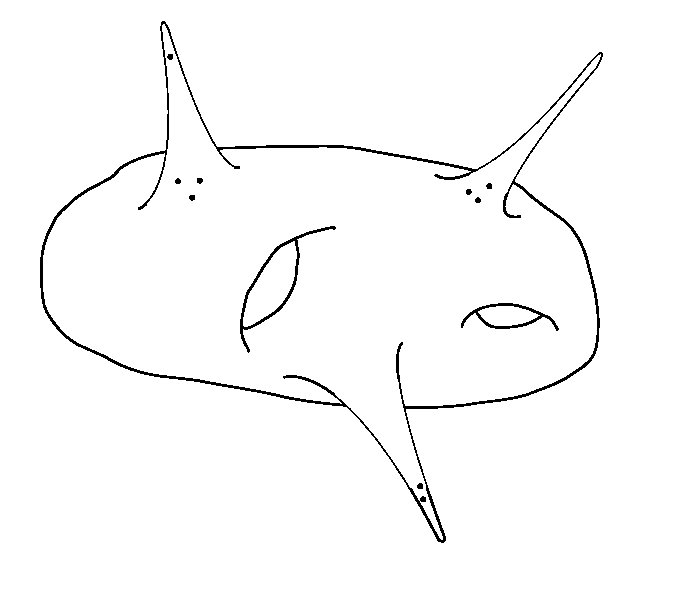
\includegraphics[width=\textwidth]{dbi/graphs/cymanifold}
 \caption[Calabi-Yau Manifold]{A representation of the Calabi-Yau manifold in the 6
compactified
dimensions. Throats are connected to the main bulk. D3-branes appear as dots.}
 \label{fig:braneworld}
\end{figure}
% 

In general, the low-energy world-volume dynamics
of a probe ${\rm D3}$-brane in a warped throat is determined 
by an effective, four-dimensional DBI action, as described in Section
\ref{sec:warpedthroats-dbiintro}.
The inflaton field is related to the radial 
position of the brane by 
$\varphi \equiv \sqrt{T_3} \rho$, where $T_3$ 
is the brane tension defined in \eq{eq:branetensiondefn-dbiintro}. The action is
then given by \cite{brane6}
% 
\begin{align}
\label{eq:DBIaction-dbiintro}
S &=\int  \d^4x \sqrt{|g|} \left[ \frac{\Mpl^2}{2} R 
+ P (\varphi , X) \right] \,,\\
\label{eq:Pdefn-dbiintro}
P( \varphi ,X) &= - T (\varphi)  \sqrt{1 - 2T^{-1} (\varphi ) X}
+T (\varphi)  -V(\varphi)  \,,
\end{align}
% 
where $R$ is the Ricci curvature scalar and $T(\varphi ) = T_3 h^4 (\varphi )$
defines the warped brane tension. As in Section \ref{sec:noncanoninfl} we refer
to $P(\varphi , X)$ as the kinetic function for the inflaton, 
$X \equiv - \frac{1}{2} g^{\mu\nu} \nabla_{\mu} \varphi \nabla_{\nu} \varphi$
is the kinetic energy of the inflaton and $V(\varphi )$ denotes 
the field's interaction 
potential. 
Typically in warped compactifications of 
IIB supergravity, this potential is determined by the 
relevant fluxes and brane interaction terms. 
We will ignore the precise origin
and form of this potential, but simply
note that it is highly sensitive to the string theoretic construction. For the
purpose of this thesis we will simply treat it 
as an arbitrary function of the inflaton field.
(See, for example, Ref. \cite{brane5} for a discussion 
on the precise form that the inflaton potential may take.)


We consider a spatially flat and isotropic cosmology 
sourced by a homogeneous scalar field. 
In this case, the Friedmann equations for a monotonically 
varying inflaton can be expressed in the form \cite{brane6} 
% 
\begin{align}
\label{eq:Friedmann-dbiintro}
3 \Mpl^2 H^2(\varphi ) &= V(\varphi ) -T(\varphi ) 
\left[ 1- \sqrt{1+4\Mpl^4T^{-1} H_{,\vp}^2} \right] \,,\\
\label{eq:phidot-useful}
\dot{\varphi} &= - \frac{2\Mpl^2H_{,\vp}}{\sqrt{1+4\Mpl^4 T^{-1} H_{,\vp}^2}}
\,.
\end{align}
% 

In Section~\ref{sec:noncanoninfl} we introduced the speed of sound of
inflaton fluctuations. For the kinetic function in
\eq{eq:Pdefn-dbiintro}, we find from
\eq{eq:defcs-dbiintro} that
% 
\begin{equation}
\label{eq:csdefn-dbiintro}
\cs = \frac{1}{P_{,X}} = \sqrt{1 -2T^{-1}X}  \,.
\end{equation}
% 
The condition that the sound speed be real 
imposes an upper bound on the kinetic energy 
of the inflaton, $\dot{\varphi}^2 < T(\varphi)$, which 
is independent of the steepness of the potential.
The motion of the brane is said to be relativistic when this bound is 
close to saturation. We will assume throughout Part~\ref{part:dbi} of this thesis that motion takes
place in the relativistic limit in which $\cs\ll1$. 
 
We now define the epoch that is directly 
accessible to cosmological observations as ``observable inflation''. 
We will assume that this phase 
occurred when the brane was located within a 
throat region and moving towards the tip of the throat. 
We denote the parameter values 
evaluated during observable inflation by a subscript star
$(~_*)$. Observable inflation corresponds to about 4 e-foldings  
of inflationary expansion, $\Delta \N_* \simeq 4$,
and occurred somewhere between 30 to 60 e-foldings before the
end of inflation. 


The definitions of the slow roll parameters defined in
Section~\ref{sec:slowroll-intro} 
change when $\cs$ is not equal to unity and we
will include a third parameter, $s$, which quantifies the rate of change of $\cs$.
The inflationary dynamics during this phase can  
be quantified in terms of these three parameters: 
% 
\begin{align}
\label{eq:epsdefn-dbiintro}
\varepsilon_H &\equiv -\frac{\dot{H}}{H^2}
= \frac{XP_{,X}}{\Mpl^2H^2} 
= \frac{2\Mpl^2}{\gamma} \left( \frac{H_{,\vp}}{H} \right)^2 \,,\\
\label{eq:defeta-dbiintro}
\eta_H &\equiv  \frac{2\Mpl^2}{\gamma}\frac{H_{,\vp\vp}}{H} \,,\\
\label{eq:defs-dbiintro}
s &\equiv \frac{\dot{\cs}}{\cs H} 
= \frac{2\Mpl^2}{\gamma} \frac{H_{,\vp}}{H}\frac{\gamma_{,\vp}}{\gamma}  \,,
\end{align}
% 
where $\gamma \equiv 1/\cs$. 
We will assume that the quasi-de Sitter conditions 
$\{ \varepsilon_H, |\eta_H | , |s | \}  \ll 1$ apply during observable inflation. 
In this regime, the amplitudes and spectral indices of the two-point functions 
for the scalar and tensor perturbations are given by \cite{gm}
% 
\begin{align}
\label{eq:spectra-dbiintro}
\Pr &= \frac{H^4}{4\pi^2\dot{\varphi}^2} =\frac{1}{8 \pi^2 \Mpl^2}
\frac{H^2}{\cs \varepsilon_H}\,,
\\
\Pt &= \frac{2}{\pi^2} \frac{H^2}{\Mpl^2} \,,
\\
\label{indices}
1-n_s &= 4 \varepsilon_H -2\eta_H  +2s \,,
\\
 n_t &= -2\varepsilon_H  \,,
\end{align}
% 
respectively. $\Pt$ and $n_t$ are evaluated when $k=aH$ but $\Pr$ and $n_s$ are
evaluated 
when the scale with wavenumber $k$ crosses 
the sound horizon $k \cs = aH$.  

A further important consequence of a small sound speed is that departures  
from purely Gaussian statistics may be large 
\cite{brane6,brane11,lidser3,chenetal}. 
DBI inflation produces non-Gaussianity maximised in the equilateral
configuration and the leading contribution is in the form of
\eq{eq:fnldefn-dbiintro}. 
When $\cs\PX=1$ the second term in 
\eq{eq:fnldefn-dbiintro} is identically zero and $\fnleq$ becomes
\cite{chenetal,lidser2}
% 
\begin{equation}
\label{eq:fnlcs-dbiintro}
\fnleq \simeq -\frac{1}{3} \left( \frac{1}{\cs^2} -1 \right) \,.
\end{equation}
% 
When $\cs\ll1$ a significant level of non-Gaussianity is produced.
% 
For a homogeneous field $2X = \dot{\vp}^2$, so from \eq{eq:csdefn-dbiintro} we
find that
\begin{equation}
\label{eq:phiT-dbiintro}
 \dot{\vp}^2 = T(\vp)(1-\cs^2)\,.
\end{equation}
Eqs. \eqref{eq:spectra-dbiintro},
\eqref{eq:fnlcs-dbiintro} and \eqref{eq:phiT-dbiintro}
may then be combined to provide a relation for the warped brane tension: 
% 
\begin{equation}
\label{eq:obswarp-dbiintro}
\frac{T (\varphi)}{\Mpl^4}  = 
\frac{\pi^2}{16} r^2\Pr \left( 1-\frac{1}{3\fnleq} \right) \,.
\end{equation}
% 


% % % % % % % % % % % % % % % % % % % % % % % % % % % % % % % % 
% =========================================================== %
% % % % % % % % % % % % % % % % % % % % % % % % % % % % % % % % 
\section{The Lyth Bound}
\label{sec:lyth-dbiintro}
% % % % % % % % % % % % % % % % % % % % % % % % % % % % % % % % 
% =========================================================== %
% % % % % % % % % % % % % % % % % % % % % % % % % % % % % % % % 
In the next two chapters we will use a powerful result due to Lyth \cite{lyth}. This
links the change in value of the inflaton field during inflation to the production of tensor
modes. This relation was originally derived for canonical actions but can be straightforwardly
extended to the case of non-canonical actions such as the DBI action.

Eqs. (\ref{eq:Ps-dbiintro}) and (\ref{eq:Ptdefn-intro}) imply 
that the variation of the inflaton field during inflation  
is related to the tensor-scalar ratio by \cite{lyth,bmpaper}
% 
\begin{equation}
\label{eq:genlyth-dbiintro}
\frac{1}{\Mpl^2}
\left( \frac{\d \varphi}{\d \N} \right)^2 = \frac{r}{8 \cs P_{,X}}
\,,
\end{equation}
% 
where $\N$ denotes the number of e-foldings as defined in
\eq{eq:nefolddefn-intro}. 
The total variation in the inflaton field between the epoch of observable 
inflation and the end of inflation is then given by
% 
\begin{equation}
\label{eq:totalfield-dbiintro}
\frac{\Delta \varphi_{\rm inf}}{\Mpl} = 
\left( \frac{r}{8 \cs P_{,X}} \right)_*^{1/2} \Neff \,,
\end{equation}
% 
where
% 
\begin{equation}
\label{eq:Neff-dbiintro}
\Neff \equiv \left( \frac{\cs P_{,X}}{r}\right)_*^{1/2}
\int_0^{\N_{\rm end}}  
\left( \frac{r}{\cs P_{,X}} \right)^{1/2} \d \N \,.
\end{equation}
% 
If $r/(\cs P_{,X})$ varies 
sufficiently slowly during observable inflation, 
the corresponding change in the value of the inflaton  
field is given approximately by \cite{lyth,bmpaper}
% 
\begin{equation}
\label{eq:approxlyth-dbiintro}
\left( \frac{\Delta \varphi}{\Mpl} \right)_*^2 \simeq 
\frac{(\Delta \N_*)^2}{8} \left( \frac{r}{\cs P_{,X}} \right)_* \,.
\end{equation}
% 
This equality links the total variation of the inflaton during observable inflation
with the tensor-scalar ratio, \iec the amplitude of gravitational waves produced
during that period. In Chapter~\ref{ch:dbi} we will show how the dynamics of the
DBI scenario allow an upper limit to be imposed on $r$ using this relation.

In deriving \eq{eq:approxlyth-dbiintro} we have assumed that $r/\cs \PX$ varies slowly during
observable inflation. For the DBI case, $\cs \PX = 1$ and the change in $r$ can be related to the
change in $\epsilon_H$ and $\cs$ through \eq{eq:rdefn-dbiintro}. As we have taken $\epsilon_H,
|\eta_H|,|s|\ll 1$ the tensor-scalar ratio will indeed vary slowly over the observable epoch.
% 
For more general models where $\cs \PX \ne 1$ we have that
% 
\begin{equation}
 \frac{\d }{\d \N}\left[ \frac{r}{\cs \PX}\right] = 16\frac{\epsilon_H}{\PX}\left( 2\epsilon_H
-2\eta_H\right)\,.
\end{equation}
% 
Therefore $r/\cs\PX$ varies slowly as long as $\PX$ is not too small, \iec close to
$\mathcal{O}(\epsilon_H^2)$. This will not be the case in the models studied in Chapters
\ref{ch:dbi} and \ref{ch:multibrane}.


% % % % % % % % % % % % % % % % % % % % % % % % % % % % % % % % 
% =========================================================== %
% % % % % % % % % % % % % % % % % % % % % % % % % % % % % % % % 
\section{Discussion}
\label{sec:summary-dbiintro}
% % % % % % % % % % % % % % % % % % % % % % % % % % % % % % % % 
% =========================================================== %
% % % % % % % % % % % % % % % % % % % % % % % % % % % % % % % % 
In this chapter we have introduced the Dirac-Born-Infeld inflationary scenario.
Many attempts have been made to provide an inflationary expansion phase in the
early universe using string theory. In compactifying from ten dimensions down to
four,
complicated geometries and additional fluxes must be used to stabilise the
remaining moduli fields. 

The DBI scenario 
is a particular example of the non-canonical inflationary para\-digm described in
Section~\ref{sec:noncanoninfl}. 
The radial position of a D3-brane in a warped throat is identified as the inflaton field. While the
brane propagates up or down the throat, the kinetic energy of the inflaton is bounded
above by requiring
the sound speed of fluctuations to be real. This bound holds no matter how steep the potential of
the field. The relativistic limit takes the bound to be close to saturation and the sound speed to
be small.
% 
In the case of DBI inflation the speed of sound
parameter
takes the simple form $\cs = 1/\PX$. The previously derived
results for $\Pr$ and $n_s$, as well as the redefined slow roll parameters 
\eqref{eq:epsdefn-dbiintro}--\eqref{eq:defs-dbiintro} can then be expressed in terms
of this parameter. 

Significant non-Gaussianity in the density perturbations spectrum can be generated
due to the small sound speed of the inflaton fluctuations.
This non-Gaussianity can be related to the brane tension and tensor-scalar ratio
through \eq{eq:obswarp-dbiintro}. The tensor-scalar ratio can also by related to the variation in
the inflaton field by the Lyth bound \eqref{eq:genlyth-dbiintro}. This relation can be refined by
focusing only on the period of observable inflation. 
% 
In the next chapter we will derive two
competing bounds on $r$ which will strongly constrain the parameter space for
DBI models.


% We will first consider the UV version of DBI inflation,
% where the brane moves relativistically 
% towards the tip of the throat. We will assume implicitly 
% that the sound speed is sufficiently small to generate a non-Gaussianity with
% magnitude in 
% excess of $|\fnl| \gtrsim 5$, since this is the projected 
% sensitivity of the Planck satellite \cite{planck}. Furthermore, we consider   
% an arbitrary warp factor and inflaton potential, 
% subject only to the condition that a sufficiently long phase of 
% quasi-exponential expansion can be maintained to solve the horizon problem of
% the hot big bang model. 
% % 
